% Example of a lycée pilote série in MIR rendering (4 exercises of the bank).
% Compile from the repo root, twice (for the sommaire):  TEXINPUTS=latex//: xelatex latex/examples/serie-pilote-corrige.tex
% Same file with \usepackage[level=1]{axiomath} (no "mir") = the coloured handout.
\documentclass[12pt,a4paper]{article}
\usepackage[level=1,mir]{axiomath}
\axsetup{title={Thalès et calcul numérique}, serie=3, classe={1\textsuperscript{ère} année -- lycée pilote}, corrige}
\begin{document}
\axmaketitle
\sommaire
\begin{rappels}
\emph{Thalès.} Si $M\in(AB)$, $N\in(AC)$ et $(MN)\parallel(BC)$, alors $\dfrac{AM}{AB}=\dfrac{AN}{AC}=\dfrac{MN}{BC}$ ;
réciproquement, si $\dfrac{AM}{AB}=\dfrac{AN}{AC}$ et si les points sont dans le même ordre, $(MN)\parallel(BC)$.
\emph{Racines.} Pour $a\geq0$, $b>0$ : $\sqrt{ab}=\sqrt a\,\sqrt b$ et $\sqrt{a/b}=\sqrt a/\sqrt b$ ; on rend un dénominateur
rationnel avec la quantité conjuguée.
\end{rappels}
\begin{corr}[title={Aires dans un trapèze}, stars=4]
$ABCD$ est un trapèze de bases $[AB]$ et $[DC]$, avec $AB=a<DC=b$. Ses diagonales se coupent en $O$. On note $S_1$, $S_2$, $S_3$ et $S_4$ les aires des triangles $OAB$, $OCD$, $OAD$ et $OBC$.

\begin{center}
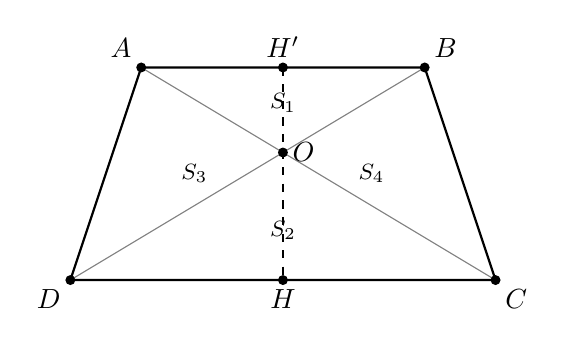
\begin{tikzpicture}[scale=0.9]
  \coordinate (D) at (0,0); \coordinate (C) at (6,0); \coordinate (A) at (1,3); \coordinate (B) at (5,3); \coordinate (O) at (3,1.8);
  \coordinate (H) at (3,0); \coordinate (Hp) at (3,3);
    \draw[thick] (A)--(B)--(C)--(D)--cycle; \draw[gray] (A)--(C); \draw[gray] (B)--(D); \draw[dashed] (Hp)--(H);
  \foreach \p/\pos in {A/above left,B/above right,C/below right,D/below left,O/right,H/below}{\fill (\p) circle (2pt) node[\pos]{$\p$};}
  \fill (Hp) circle (2pt) node[above]{$H'$};
  \node at (3,2.5) {\footnotesize$S_1$}; \node at (3,0.7) {\footnotesize$S_2$}; \node at (1.75,1.5) {\footnotesize$S_3$}; \node at (4.25,1.5) {\footnotesize$S_4$};
\end{tikzpicture}
\end{center}
\begin{enumerate}
  \item Montrer que $\dfrac{OA}{OC}=\dfrac{OB}{OD}=\dfrac ab$.
  \item La perpendiculaire à $(AB)$ passant par $O$ coupe $(AB)$ en $H'$ et $(DC)$ en $H$. Montrer que $\dfrac{OH'}{OH}=\dfrac ab$, puis que $\dfrac{S_1}{S_2}=\dfrac{a^2}{b^2}$.
  \item Montrer que $S_3=S_4$. [Comparer les aires de $ABD$ et de $ABC$.]
  \item Montrer que $\dfrac{S_3}{S_1}=\dfrac ba$, puis que $S_3^{\,2}=S_1\,S_2$.
  \item En déduire que l'aire du trapèze est $\big(\sqrt{S_1}+\sqrt{S_2}\big)^2$.
  \item Application : $S_1=16$ et $S_2=25$. Calculer $S_3$, l'aire du trapèze et le rapport $\dfrac ab$.
\end{enumerate}
\axsol
\begin{prop}[Papillon et aires]
Deux droites se coupent en $O$, avec $(AB)\parallel(CD)$ : on part du sommet $O$, \ib{$\dfrac{OA}{OC}=\dfrac{OB}{OD}=\dfrac{AB}{CD}$}.

Aire d'un triangle : \ib{$\dfrac12\times\text{base}\times\text{hauteur}$}. Deux triangles de \textbf{même base} et de \textbf{même hauteur} ont la même aire ; deux triangles de \textbf{même hauteur} ont des aires proportionnelles à leurs bases.
\end{prop}
\begin{enumerate}
  \item Les droites $(AC)$ et $(BD)$ se coupent en $O$ et $(AB)\parallel(DC)$. Papillon de sommet $O$ (triangles $OAB$ et $OCD$) :
  \[\dfrac{OA}{OC}=\dfrac{OB}{OD}=\dfrac{AB}{CD}=\ib{$\dfrac ab$}\]

  \item Les droites $(AC)$ et $(H'H)$ se coupent en $O$. Comme $(AB)\parallel(DC)$, la perpendiculaire à $(AB)$ est aussi perpendiculaire à $(DC)$, et $(AH')\parallel(CH)$. Papillon de sommet $O$ :
  \[\dfrac{OH'}{OH}=\dfrac{OA}{OC}=\dfrac ab\]
  $OH'$ est la hauteur de $OAB$ et $OH$ celle de $OCD$ :
  \[S_1=\dfrac12\,a\times OH'\qquad S_2=\dfrac12\,b\times OH\]
  \[\dfrac{S_1}{S_2}=\dfrac ab\times\dfrac{OH'}{OH}=\dfrac ab\times\dfrac ab=\ib{$\dfrac{a^2}{b^2}$}\]

  \item Les triangles $ABD$ et $ABC$ ont la même base $[AB]$ et la même hauteur (la distance entre les parallèles $(AB)$ et $(DC)$) : ils ont la même aire.

  Or $\text{aire}(ABD)=S_1+S_3$ et $\text{aire}(ABC)=S_1+S_4$. Donc
  \[S_1+S_3=S_1+S_4\implies\ib{$S_3=S_4$}\]

  \item Les triangles $OAD$ et $OAB$ ont le même sommet $A$ et leurs bases $[OD]$ et $[OB]$ sont sur la même droite $(BD)$ : même hauteur issue de $A$.
  \[\dfrac{S_3}{S_1}=\dfrac{OD}{OB}=\ib{$\dfrac ba$}\]
  (car $\dfrac{OB}{OD}=\dfrac ab$ d'après la question 1). On exprime $S_3$ et $S_2$ avec $S_1$ :
  \[S_3=\dfrac ba\,S_1\qquad S_2=\dfrac{b^2}{a^2}\,S_1\ \ \text{(question 2)}\]
  \[S_1\,S_2=\dfrac{b^2}{a^2}\,S_1^{\,2}=\left(\dfrac ba\,S_1\right)^2=S_3^{\,2}\]

  \item L'aire du trapèze est la somme des quatre triangles :
  \[S=S_1+S_2+S_3+S_4=S_1+S_2+2S_3\]
  Comme $S_3>0$ et $S_3^{\,2}=S_1S_2$, on a $S_3=\sqrt{S_1}\sqrt{S_2}$ :
  \[S=S_1+S_2+2\sqrt{S_1}\sqrt{S_2}=\ib{$\big(\sqrt{S_1}+\sqrt{S_2}\big)^2$}\]

  \item $S_3=\sqrt{16\times25}=\sqrt{400}=\boxed{20}$ et :
  \[S=(\sqrt{16}+\sqrt{25})^2=(4+5)^2=\ib{$81$}\]
  Contrôle : $16+25+20+20=81$.

  Le rapport $\dfrac ab$ vérifie $\dfrac{a^2}{b^2}=\dfrac{S_1}{S_2}=\dfrac{16}{25}$, donc $\dfrac ab=\boxed{\dfrac45}$.
\end{enumerate}
\textbf{Idée :} deux triangles de même base et de même hauteur ont la même aire, et un papillon de rapport $k$ multiplie les aires par $k^2$.

\textbf{Piège :} écrire $\dfrac{S_1}{S_2}=\dfrac ab$ (rapport des aires et non des longueurs), ou croire que les quatre triangles ont la même aire.
\end{corr}

\begin{corr}[title={Une droite par le centre de gravité}, stars=4]
$ABC$ est un triangle, $I$ le milieu de $[BC]$ et $G$ le point de $[AI]$ tel que $AG=\dfrac23AI$. Une droite $d$ passant par $G$, mais pas par $A$, coupe $[AB]$ en $M$ et $[AC]$ en $N$. Les parallèles à $d$ passant par $B$ et par $C$ coupent la droite $(AI)$ en $U$ et $V$ ; on admet que $U$ et $V$ sont sur la demi-droite $[AI)$, au-delà de $G$.

\begin{center}
\begin{tikzpicture}[scale=1.15]
  \coordinate (A) at (3,6); \coordinate (B) at (0,0); \coordinate (C) at (9,0); \coordinate (I) at (4.5,0); \coordinate (G) at (4,2);
  \coordinate (M) at (0.75,1.5); \coordinate (N) at (6.6,2.4); \coordinate (U) at (4.3333,0.6667); \coordinate (V) at (4.6667,-0.6667);
  \draw[thick] (A)--(B)--(C)--cycle; \draw[gray] (A)--(V);
  \draw[thick] ($(M)!-0.35!(N)$)--($(N)!-0.25!(M)$);
  \draw[dashed] (B)--(U); \draw[dashed] (C)--(V);
  \foreach \p/\pos in {A/above,B/below left,C/below right,I/above left,G/above left,M/left,N/right,U/above right,V/below right}{\fill (\p) circle (2pt) node[\pos]{$\p$};}
  \node[axmain] at (-0.55,1.25) {$d$};
\end{tikzpicture}
\end{center}
\begin{enumerate}
  \item Montrer que $I$ est le milieu de $[UV]$, puis que $AU+AV=2\,AI$. [Papillon de sommet $I$ dans les triangles $IBU$ et $ICV$.]
  \item Écrire Thalès de sommet $A$ dans les triangles $ABU$ et $ACV$ pour montrer que $\dfrac{AB}{AM}=\dfrac{AU}{AG}$ et $\dfrac{AC}{AN}=\dfrac{AV}{AG}$.
  \item En déduire que $\dfrac{AB}{AM}+\dfrac{AC}{AN}=3$.
  \item Application : $AB=12$, $AC=10$ et $AM=9$. Calculer $AN$. Que devient la relation lorsque $d\parallel(BC)$ ? lorsque $d=(BG)$ ?
  \item On pose $x=\dfrac{AM}{AB}$, $y=\dfrac{AN}{AC}$ et on note $\mathcal S$ l'aire de $ABC$. Montrer que $\text{aire}(AMN)=xy\,\mathcal S$, puis que $\dfrac49\,\mathcal S\leq\text{aire}(AMN)\leq\dfrac12\,\mathcal S$. Préciser les positions de $d$ pour lesquelles il y a égalité. [Poser $u=\dfrac1x$ ; montrer que $1\leq u\leq2$ et que $xy=\dfrac1{u(3-u)}$.]
\end{enumerate}
\axsol
\begin{prop}[Thalès et papillon]
\textbf{Triangle.} $M\in[AB]$, $G\in[AU]$, $(MG)\parallel(BU)$ : on part de $A$, \ib{$\dfrac{AM}{AB}=\dfrac{AG}{AU}=\dfrac{MG}{BU}$}.

\textbf{Papillon.} Deux droites se coupent en $I$, avec $(BU)\parallel(CV)$ : on part de $I$, \ib{$\dfrac{IB}{IC}=\dfrac{IU}{IV}=\dfrac{BU}{CV}$}.
\end{prop}
\begin{enumerate}
  \item Les droites $(BC)$ et $(UV)=(AI)$ se coupent en $I$. Les droites $(BU)$ et $(CV)$ sont parallèles (toutes deux parallèles à $d$). Papillon de sommet $I$ (triangles $IBU$ et $ICV$) :
  \[\dfrac{IB}{IC}=\dfrac{IU}{IV}=\dfrac{BU}{CV}\]
  $I$ est le milieu de $[BC]$ : $IB=IC$, donc $IU=IV$. Les points $B$ et $C$ sont de part et d'autre de $I$, donc $U$ et $V$ aussi : \ib{$I$ est le milieu de $[UV]$}.

  Les points $U$ et $V$ sont sur la même demi-droite d'origine $A$. Sur cette demi-droite, le milieu de $[UV]$ est à la distance $\dfrac{AU+AV}2$ de $A$ :
  \[AI=\dfrac{AU+AV}2\implies\ib{$AU+AV=2\,AI$}\]

  \item \textbf{Triangle $ABU$.} On a $M\in[AB]$, $G\in[AU]$ (car $U$ est au-delà de $G$) et $(MG)=d\parallel(BU)$. Thalès de sommet $A$ :
  \[\dfrac{AM}{AB}=\dfrac{AG}{AU}\implies\ib{$\dfrac{AB}{AM}=\dfrac{AU}{AG}$}\]
  \textbf{Triangle $ACV$.} On a $N\in[AC]$, $G\in[AV]$ et $(NG)=d\parallel(CV)$. Thalès de sommet $A$ :
  \[\dfrac{AN}{AC}=\dfrac{AG}{AV}\implies\ib{$\dfrac{AC}{AN}=\dfrac{AV}{AG}$}\]

  \item On additionne les deux égalités de la question 2 :
  \[\dfrac{AB}{AM}+\dfrac{AC}{AN}=\dfrac{AU+AV}{AG}=\dfrac{2\,AI}{AG}\]
  Comme $AG=\dfrac23AI$ :
  \[\dfrac{AB}{AM}+\dfrac{AC}{AN}=\dfrac{2\,AI}{\frac23AI}=\ib{$3$}\]

  \item \textbf{Application.} $\dfrac{12}9+\dfrac{10}{AN}=3\implies\dfrac{10}{AN}=3-\dfrac43=\dfrac53\implies AN=\boxed{6}$.

  \textbf{Si $d\parallel(BC)$.} Thalès de sommet $A$ dans $ABI$ (avec $G\in[AI]$) donne $\dfrac{AM}{AB}=\dfrac{AG}{AI}=\dfrac23$ ; de même $\dfrac{AN}{AC}=\dfrac23$. On retrouve $\dfrac32+\dfrac32=3$.

  \textbf{Si $d=(BG)$.} Alors $M=B$ et $\dfrac{AB}{AM}=1$. La relation donne $\dfrac{AC}{AN}=2$ : $N$ est le milieu de $[AC]$ (la droite $(BG)$ est la médiane issue de $B$).

  \item \textbf{Les aires.} Les triangles $AMN$ et $ABN$ ont le même sommet $N$ et leurs bases $[AM]$ et $[AB]$ sont sur la même droite : même hauteur, donc
  \[\dfrac{\text{aire}(AMN)}{\text{aire}(ABN)}=\dfrac{AM}{AB}=x\]
  De même, $ABN$ et $ABC$ ont le même sommet $B$ et leurs bases $[AN]$ et $[AC]$ sont sur la droite $(AC)$ :
  \[\dfrac{\text{aire}(ABN)}{\text{aire}(ABC)}=\dfrac{AN}{AC}=y\]
  \[\text{aire}(AMN)=xy\,\mathcal S\]
  \textbf{La relation.} La question 3 s'écrit $\dfrac1x+\dfrac1y=3$. On pose $u=\dfrac1x$ et $v=\dfrac1y=3-u$.

  Comme $0<x\leq1$ et $0<y\leq1$ : $u\geq1$ et $v\geq1$, donc $3-u\geq1$, c'est-à-dire $1\leq u\leq2$.
  \[xy=\dfrac1{uv}=\dfrac1{u(3-u)}\]
  \textbf{Encadrement de $u(3-u)$.} On écrit
  \[u(3-u)=\dfrac94-\left(u-\dfrac32\right)^2\]
  Pour $1\leq u\leq2$ : $0\leq\left(u-\dfrac32\right)^2\leq\dfrac14$, donc
  \[2\leq u(3-u)\leq\dfrac94\implies\dfrac49\leq xy\leq\dfrac12\]
  \[\ib{$\dfrac49\,\mathcal S\leq\text{aire}(AMN)\leq\dfrac12\,\mathcal S$}\]
  \textbf{Cas d'égalité.} $xy=\dfrac49$ si et seulement si $u=\dfrac32$, c'est-à-dire $x=y=\dfrac23$ : $d$ est parallèle à $(BC)$.

  $xy=\dfrac12$ si et seulement si $\left(u-\dfrac32\right)^2=\dfrac14$, c'est-à-dire $u=1$ ou $u=2$ : $M=B$ et $N$ milieu de $[AC]$ (la médiane $(BG)$), ou bien $N=C$ et $M$ milieu de $[AB]$ (la médiane $(CG)$).
\end{enumerate}
\textbf{Idée :} les deux parallèles à $d$ menées par $B$ et $C$ transportent les rapports $\dfrac{AB}{AM}$ et $\dfrac{AC}{AN}$ sur la droite $(AI)$, où le milieu $I$ les fait s'additionner.

\textbf{Piège :} écrire Thalès dans le triangle $ABC$ : la droite $(MN)$ n'est pas parallèle à $(BC)$ en général.
\end{corr}

\begin{corr}[title={Racines irrationnelles}, stars=4]
Un nombre est \emph{rationnel} s'il s'écrit $\dfrac pq$ avec $p$, $q$ entiers, $q\neq0$, la fraction étant irréductible ($p$ et $q$ n'ont pas de diviseur commun autre que $1$).
\begin{enumerate}
  \item Montrer que si le carré d'un entier $n$ est pair, alors $n$ est pair. [Étudier le cas $n$ impair.]
  \item On suppose que $\sqrt2=\dfrac pq$ (fraction irréductible). Montrer que $p^2=2q^2$, puis que $p$ et $q$ sont pairs. Conclure que $\sqrt2$ n'est pas rationnel.
  \item Montrer de même que $\sqrt6$ n'est pas rationnel.
  \item En calculant $(\sqrt2+\sqrt3)^2$, montrer que $\sqrt2+\sqrt3$ n'est pas rationnel.
  \item En déduire que $\sqrt3-\sqrt2$ n'est pas rationnel.
\end{enumerate}
\axsol
\begin{prop}[Raisonnement par l'absurde]
Pour montrer qu'une propriété est vraie, on suppose qu'elle est \textbf{fausse} et on aboutit à une \ib{contradiction}. Un entier est pair s'il s'écrit $2m$, impair s'il s'écrit $2m+1$ ; le produit de deux entiers impairs est impair.
\end{prop}
\begin{enumerate}
  \item On montre : \og $n$ impair $\implies n^2$ impair \fg{}.

  Si $n=2m+1$ :
  \[n^2=4m^2+4m+1=2\,(2m^2+2m)+1\]
  $n^2$ est impair. Donc, si $n^2$ est pair, $n$ ne peut pas être impair : \textbf{$n$ est pair}.

  \item On élève $\sqrt2=\dfrac pq$ au carré : $2=\dfrac{p^2}{q^2}$, soit
  \[p^2=2q^2\]
  Donc $p^2$ est pair, et d'après la question 1, $p$ est pair : $p=2m$.

  On remplace : $4m^2=2q^2$, donc
  \[q^2=2m^2\]
  Donc $q^2$ est pair, et $q$ est pair.

  $p$ et $q$ sont tous deux pairs : $2$ est un diviseur commun, ce qui contredit \og fraction irréductible \fg{}. L'hypothèse est fausse :
  \[\ib{$\sqrt2$ n'est pas rationnel}\]

  \item On suppose $\sqrt6=\dfrac pq$ (irréductible). Alors $p^2=6q^2$ : $p^2$ est pair, donc $p=2m$.

  On remplace : $4m^2=6q^2$, soit
  \[2m^2=3q^2\]
  Le nombre $3q^2$ est pair. Si $q^2$ était impair, $3q^2$ serait un produit de deux impairs, donc impair : c'est faux. Donc $q^2$ est pair, et $q$ est pair.

  $p$ et $q$ sont pairs : contradiction. \ib{$\sqrt6$ n'est pas rationnel.}

  \item On développe :
  \[(\sqrt2+\sqrt3)^2=2+2\sqrt6+3=5+2\sqrt6\]
  Supposons $\sqrt2+\sqrt3=r$ rationnel. Alors $r^2=5+2\sqrt6$, donc
  \[\sqrt6=\dfrac{r^2-5}2\]
  Ce nombre est rationnel (opérations sur des rationnels) : cela contredit la question 3.

  \ib{$\sqrt2+\sqrt3$ n'est pas rationnel.}

  \item On calcule le produit conjugué :
  \[(\sqrt3-\sqrt2)(\sqrt3+\sqrt2)=3-2=1\implies\sqrt3-\sqrt2=\dfrac1{\sqrt3+\sqrt2}\]
  Supposons $\sqrt3-\sqrt2=s$ rationnel. Comme $s>0$, $\sqrt3+\sqrt2=\dfrac1s$ serait rationnel : cela contredit la question 4.

  \ib{$\sqrt3-\sqrt2$ n'est pas rationnel.}
\end{enumerate}
\textbf{Idée :} supposer le contraire et chercher un diviseur commun caché dans la fraction \og irréductible \fg{}.

\textbf{Piège :} pour $\sqrt6$, on aboutit à $2m^2=3q^2$ : il faut encore justifier que $q$ est pair (le facteur $3$ est impair).
\end{corr}

\begin{corr}[title={PGCD et divisibilité par 2, 4, 8}, stars=4]
Pour tout entier naturel $n$, on pose $d_n=\mathrm{PGCD}(n+2,\ n^2+4)$.
\begin{enumerate}
  \item Calculer $d_n$ pour $n=0,1,2,\dots,8$.
  \item Montrer que $n^2+4=(n+2)(n-2)+8$. En déduire que $d_n=\mathrm{PGCD}(n+2,\ 8)$.
  \item Montrer que $d_n=1$ si $n$ est impair, $d_n=2$ si $n$ est multiple de $4$, $d_n=4$ si $n=8q+2$ et $d_n=8$ si $n=8q+6$.
  \item Calculer $d_{2026}$ et $d_{2030}$.
\end{enumerate}
\axsol
\begin{prop}[PGCD]
Pour tous entiers $a$, $b$ et $q$ : \ib{$\mathrm{PGCD}(a,b)=\mathrm{PGCD}(b,\,a-qb)$}. Les diviseurs de $8$ sont $1$, $2$, $4$ et $8$.
\end{prop}
\begin{enumerate}
  \item On calcule les couples $(n+2,\,n^2+4)$ :
  \[\begin{array}{c|ccccccccc}
  n&0&1&2&3&4&5&6&7&8\\\hline
  (n+2,\,n^2+4)&(2,4)&(3,5)&(4,8)&(5,13)&(6,20)&(7,29)&(8,40)&(9,53)&(10,68)\\\hline
  d_n&2&1&4&1&2&1&8&1&2
  \end{array}\]

  \item On développe :
  \[(n+2)(n-2)+8=n^2-4+8=n^2+4\]
  On applique la propriété du PGCD avec $a=n^2+4$, $b=n+2$ et $q=n-2$ :
  \[a-qb=(n^2+4)-(n-2)(n+2)=8\]
  \[d_n=\mathrm{PGCD}(n+2,\ n^2+4)=\ib{$\mathrm{PGCD}(n+2,\ 8)$}\]
  (Un diviseur commun de $a$ et $b$ divise $a-qb$ ; réciproquement un diviseur commun de $b$ et $a-qb$ divise $a=(a-qb)+qb$.)

  \item Le PGCD est un diviseur de $8$ : c'est le plus grand élément de $\{1,2,4,8\}$ qui divise $n+2$.

  \textbf{$n$ impair.} $n+2$ est impair : ni $2$, ni $4$, ni $8$ ne le divisent. Donc $d_n=\boxed{1}$.

  \textbf{$n=4q$.} $n+2=4q+2=2\,(2q+1)$ : divisible par $2$, mais pas par $4$ (le reste de la division par $4$ est $2$). Donc $d_n=\boxed{2}$.

  \textbf{$n=8q+2$.} $n+2=8q+4=4\,(2q+1)$ : divisible par $4$, mais pas par $8$ (le reste de la division par $8$ est $4$). Donc $d_n=\boxed{4}$.

  \textbf{$n=8q+6$.} $n+2=8q+8=8\,(q+1)$ : divisible par $8$. Donc $d_n=\boxed{8}$.

  Ces quatre cas épuisent tous les entiers : un entier pair est de la forme $8q$, $8q+2$, $8q+4$ ou $8q+6$, et $8q$ et $8q+4$ sont des multiples de $4$. Le tableau de la question 1 est cohérent ($d_6=8$, $d_2=4$, $d_0=d_4=d_8=2$).

  \item $2026=8\times253+2$ : on est dans le cas $n=8q+2$.
  \[d_{2026}=\ib{$4$}\qquad(2028=4\times507\ \text{et}\ 2028=8\times253+4)\]
  $2030=8\times253+6$ : on est dans le cas $n=8q+6$.
  \[d_{2030}=\ib{$8$}\qquad(2032=8\times254)\]
\end{enumerate}
\textbf{Idée :} le reste $8$ de la division de $n^2+4$ par $n+2$ ramène le problème à des critères de divisibilité par $2$, $4$ et $8$.

\textbf{Piège :} croire que $d_n=1$ pour tout $n$ (par exemple $d_6=8$).
\end{corr}

\end{document}
